\documentclass[a4paper,10pt]{article}
\usepackage[T1]{fontenc}        % Codifica dei font
\usepackage[utf8]{inputenc}    % Lettere accentate da tastiera
\usepackage[english,italian]{babel}     % Lingua del documento
\usepackage{color, colortbl}
\usepackage{booktabs}
\usepackage{array}
%\usepackage[compact]{titlesec}
\usepackage[margin=0.8in, includefoot]{geometry}
\usepackage{longtable}
\usepackage{graphicx}
\usepackage{amssymb}


\newcolumntype{P}[1]{>{\centering\arraybackslash}p{#1}}
\newcolumntype{S}[1]{>{\arraybackslash}p{#1}}
%\titleformat{\chapter}[display]{\bfseries}{}{-30pt}{\Huge}

\renewcommand{\familydefault}{\sfdefault}
\usepackage[scaled]{helvet}
\begin{document}
\title{%
    Progetto per il corso di Basi di Dati \\
    \large LT in Informatica, Universita degli studi di Padova}
\author{Niccolò Mantovani, 1234567
    \and
    Filippo Pinton, 1234567}
\date{}

\maketitle

\tableofcontents

\section{Abstract}
Storia antica quasi 10000 anni 

Fa parte della cultura (religiosa e non) di moltissimi

Italia maggiore esportatore di vino al mondo

Fatturato +7.5 nel 2018 

Il fatturato maggiore lo hanno due colossi cooperativi -> cooperative -> e' un ambiente spesso gestito da piccole aziende agricole 
con poche risorse e talvolta poca/arretrata organizzazione

Descrizione societa' fittizia 


\section{Analisi dei requisiti}
%\section{introduzione}
 %   Introduzione all'analisi dei requisiti

%\section{considerazioni}
 %   Considerazioni
 
%  L'interesse principale di questo progetto e' modellare una base di dati che supporti l'operativita' della cantina vinicola \emph{NomeCantina}. La principale merce prodotta e' la \textbf{bottiglia di vino} che rappresenta l'unione di una bottiglia di vetro, di un tappo e di un tipo di vino. Ogni bottiglia è identificata dal nome del vino e dall'annata di esso. Dati importanti per tale prodotto sono il prezzo, il numero di unità prodotte e vendute, oltre che dal tipo di tappo e dal tipo di bottiglia.
Altro prodotto importante è il \textbf{vino}, che viene identificato tramite il nome. Inoltre dati importanti del vino sono la gradazione alcolica, il tempo di fermentazione e l'uva utilizzata oltre che lo stato produttivo, ovvero se il vino viene prodotto ancora o è ormai fuori commercio. Importante registrare la classificazione del vino: vini a denominazione d'origine controllata e garantita (D.O.C.G.); vini a denominazione d'origine controllata (D.O.C.); vini ad indicazione geografica tipica (I.G.T.).\\ Ovviamente la cantina acquista esternamente da altre aziende le proprie materie prime che vanno a formare il prodotto finale. Le \textbf{materie prime} che vengono acquistate vengono identificate con un ID univoco. Se la materia prima è l'uva questa viene rappresentata dall'anno di raccolta, dal nome e dal colore. Se, invece, la materia prima sono i tappi questa viene rappresentata dalla forma e dal materiale, infine se la materia prima sono le bottiglie, questa viene rappresentata dalla capacità e dal colore. Inoltre è presente il dato che identifica la quantità posseduta dalla cantina sia per i tappi che per le bottigle.\\
Un tipo d'uva proviene da un tipo di \textbf{vigneto}, rappresentato da un ID univoco e dalla loro posizione geografica. \\
Le aziende con cui la cantina ha relazione sono molteplici. Queste \textbf{aziende} si dividono in fornitori, aziende di manutenzione macchinari e negozi interni della cantina. Le aziende sono identificate tramite un ID univoco e sono caratterizzate dal nome, dalla Partita IVA, dal nome e dal cognome del referente oltre che dal numero di telefono, dalla email aziendale e dalla sua posizione geografica (che corrisponde con l'indirizzo di spedizione). Per le aziende che sono fornitori rappresentiamo poi la tipologia di materia prima fornita, sia essa uva, tappi o bottiglie.\\
Ovviamente le bottiglie di vino possono essere spedite in una determinata quantità in un \textbf{ordine} di vendita. Relativamente ad un ordine rappresentiamo un ID univoco, la data in cui è stato effettuato, il \textbf{corriere} (rappresentato tramite un ID ed un nome commerciale.) a cui è stata affidato, la data di spedizione, la data di consegna e il prezzo totale (che deve corrispondere al prodotto tra il prezzo delle bottiglie di vino acquistate e il relativo prezzo sommato al costo della spedizione).\\
Ogni ordine viene venduto ad un acquirente, che può essere un'azienda o un \textbf{privato}. Per i privati, identificati da un ID, rappresentiamo il nome, il cognome, il numero di telefono e l'email oltre che l'indirizzo di residenza (che corrisponde con l'indirizzo di spedizione).\\
E' di consuetudine, per la cantina \emph{NomeCantina}, organizzare degli eventi all'interno dei propri negozi. Gli \textbf{eventi} hanno una tematica che è rappresentata da un nostro vino e vengono definiti tramite il titolo dell'evento e il numero di edizione. Ovviamente ogni evento ha una data prefissata in cui si svolgerà.
Riguardo al reparto produttivo sono presenti tutte le tipologie di lavorazione dell'uva per la produzione del vino. Queste \textbf{linee produttive} sono l'ingresso delle materie prime, la pigiatura, la fermentazione, la vinificazione e la svinatura. Oltre a queste esistono altri reparti produttivi come l'imbottigliamento e il magazzino dove le bottiglie di vino vengono divise per la colorazione del proprio vino (rosso, bianco, rosato e spumante).Nel magazzino viene tenuto traccia della quantità delle bottiglie. Tutti questi reparti sono identificati tramite un identificativo.\\
In ognugno di questi reparti lavorano dei \textbf{dipendeti} in determinati turni di lavoro. Per ogni dipendete (identificato tramite il codice fiscale) viene registrato il nome e il cognome. Ogni dipendente avrà un supervisore a cui fare riferimento e ogni linea produttiva sarà diretta da un dipendente dell'azienda.\\
Per ogni linea produttiva sono presenti dei \textbf{macchinari} che aiutano i dipendenti nelle mansioni quotidiane. I macchinari sono identificati tramite un codice univoco. Ad ogni macchinario viene fatta una manutenzione periodica, quindi è utile tenere traccia della data della prossima manutenzione. I macchinari avranno anche un nome commerciale e la data di acquisto.\\
Le manutenzioni avranno un costo e verrano eseguite in una determinata data. Le manutenzioni vengono eseguite da aziende esterne rappresentate come sopra.
    
  \subsection{Glossario dei termini}
    \subsubsection{Considerazioni su Bottiglia di Vino}
Considerazioni

\begin{center}
	\begin{longtable}{P{2cm}P{2cm}P{6cm}P{4cm}}
		\toprule
		\rowcolor[rgb]{.929, .929, .929} Termine & Sinonimi & Descrizione & Collegamento \\
		
		\midrule
		Bottiglia di vino & & Una bottiglia di vino della cantina in vendita online e nei negozi fisici. & Vino, Bottiglia, Tappo, Ordine, Magazzino\\
		\midrule
		Vino & Tipo Vino & Le tipologie di vino prodotte all'interno della cantina. & Uva, Evento, Bottiglia di vino \\
		
		\midrule
		Materia prima & & Rappresenta le materie prime che vengono acquistate e manipolate per comporre le bottiglie di vino. &  Vino, Tipo Uva, Fornitore, Bottiglia di vino\\
		
		\midrule
		Uva & Tipo Uva & La tipologia dell'uva che viene acquistata per produrre il vino. &  Vigneto, Vino\\
		
		\midrule
		Vigneto & & Rappresenta il vigneto dalla quale proviene un determinato lotto di uva acquistato. &  Tipo Uva\\

		\midrule
		Acquirente & Privato, Azienda & Colui che ha effettuato l'ordine. Può essere un privato o un'azienda &  Ordine\\

		\midrule
		Azienda & Fornitore, Negozio interno, A. Manutenz. & Un'azienda con cui la cantina ha rapporti, siano questi di fornitura, di vendita o di altra natura. &  Materia prima, Evento, Macchinario\\

		\midrule
		Ordine & & Un ordine effettuato da un acquirente, contiene le informazioni della merce acquistata e della spedizione. &  Bottiglia di vino, Corriere, Acquirente\\
		
		\midrule
		Corriere & & Il corriere che si occupa della spedizione di un ordine & Ordine\\
		\midrule
		
		Evento & & Un evento organizzato all'interno di un negozio interno in onore di un vino prodotto dalla cantina. &  Tipo Vino, Negozio Interno\\

		\midrule
		Linea produttiva & & Un reparto produttivo interno alla cantina. &  Dipendente, Macchinario\\

		\midrule
		Dipendente & & Colui che lavora per la cantina ed è assegnato ad una linea produttiva &  Linea produttiva\\

		\midrule
		Macchinario & & Strumento utilizzato all'interno di una linea produttiva &  Linea produttiva, Azienda manutenzione\\
		
		\bottomrule
	\end{longtable}
\end{center}
   
  \subsection{Operazioni Tipiche}
    \begin{center}
	\begin{tabular}{P{9.5cm}P{6cm}}
		\toprule
		\rowcolor[rgb]{.929, .929, .929} Operazione & Frequenza \\
		\midrule
		Vendita ordine & 1000 volte al giorno\\
		\midrule
		Acquisto materie prime & 2 volte all'anno\\
		\midrule
		Manutenzione macchinari & 200 volte all'anno\\
		\midrule
		Organizzazione eventi & 5 volte all'anno\\
		\midrule
		Inserimento dipendente & 30 volte all'anno\\
		\midrule
		Inserimento turno & 30 volte al giorno\\
		\midrule
		Inserimento acquirente & 1 volta al mese\\
		\bottomrule
	\end{tabular}
\end{center}
   
  \subsection{Strutturazione dei requisiti}
    \begin{center}
	\begin{tabular}{P{16cm}}
		\toprule
		\rowcolor[rgb]{.929, .929, .929} \textbf {\large {FRASI RELATIVE A BOTTIGLIA DI VINO}} \\
		\midrule
		La bottiglia di vino che è caratterizzata dal tipo di vino contenuto e dall'annata. Altri dati importanti sono il prezzo per bottiglia, il numero di bottiglie prodotte e vendute, il tipo di tappo e bottiglia ed infine dalla classificazione: vini a denominazione d'origine controllata e garantita (D.O.C.G.); vini a denominazione d'origine controllata (D.O.C.); vini ad indicazione geografica tipica (I.G.T.). Ciascuna tipologia di bottiglia di vino è racchiusa in magazzini. Ovviamente le bottiglie di vino possono essere spedite in una determinata quantità in un ordine di vendità\\
		\bottomrule
	\end{tabular}

	\vspace{0.5cm}
	
	\begin{tabular}{P{16cm}}
		\toprule
		\rowcolor[rgb]{.929, .929, .929} \textbf {\large {FRASI RELATIVE A VINO}} \\
		\midrule
		Altro prodotto importante è il vino, che viene identificato tramite il nome. Inoltre dati importanti del vino sono la gradazione alcolica, il tempo di fermentazione, la tipologia di uva con cui è stata prodotta, caratterizzata dalla vedemmia (data raccolta) e dal colore.  Importante inoltre tenere traccia se un determinato vino è ancora in fase di produzione o è diventato fuori commercio.\\
		\bottomrule
	\end{tabular}

	\vspace{0.5cm}
	
	\begin{tabular}{P{16cm}}
		\toprule
		\rowcolor[rgb]{.929, .929, .929} \textbf {\large {FRASI RELATIVE AD UVA}} \\
		\midrule
		la tipologia di uva con cui è stata prodotta, caratterizzata dalla vedemmia (data raccolta) e dal colore. L'uva viene identificata tramite la tipologia e la vendemmia. L'uva proviene da un tipo di vigna\\
		\bottomrule
	\end{tabular}

	\vspace{0.5cm}

	\begin{tabular}{P{16cm}}
		\toprule
		\rowcolor[rgb]{.929, .929, .929} \textbf {\large {FRASI RELATIVE A VIGNA}} \\
		\midrule
		L'uva proviene da un tipo di vigna, identificata da un ID, la quale è coltivata in un determinato vigneto. Importante identificare la data della piantagione della vigna.\\
		\bottomrule
	\end{tabular}

	\vspace{0.5cm}
	
	\begin{tabular}{P{16cm}}
		\toprule
		\rowcolor[rgb]{.929, .929, .929} \textbf {\large {FRASI RELATIVE A VIGNETO}} \\
		\midrule
		Del vigneto, anch'esso identificato tramite un ID è utile identificatore l'indirizzo di locazione e il tipo di terreno di piantagione.\\
		\bottomrule
	\end{tabular}
	
	\vspace{0.5cm}
	
	\begin{tabular}{P{16cm}}
		\toprule
		\rowcolor[rgb]{.929, .929, .929} \textbf {\large {FRASI RELATIVE A FORNITORE}} \\
		\midrule
		L'uva è fornita da aziende esterne. Alcune di queste aziende fanno comunque parte del gruppo \emph{Nome Cantina}, ma sono gestite esternamente. Esistono fornitori di uva, bottglie e tappi.
I fornitori sono identificati tramite un identificativo univoco. Inoltre hanno un nome commerciale e hanno il loro prezzo per prodotto; specificatamente hanno il prezzo al Kg per i fornitori di uva e prezzo al prodotto (tappo o bottiglia) per le altre due tipologie di fornitori. Per ogni fornitura va identificata la data, il prezzo e la quantità del prodotto fornito\\
		\bottomrule
	\end{tabular}
	
	\vspace{0.5cm}
	
	\begin{tabular}{P{16cm}}
		\toprule
		\rowcolor[rgb]{.929, .929, .929} \textbf {\large {FRASI RELATIVE A TAPPO}} \\
		\midrule
		I tappi vengono rappresentati tramite la forma ed il materiale. Inoltre è presente il dato che identifica la quantità posseduta dalla cantina per i tappi\\
		\bottomrule
	\end{tabular}
	
	\vspace{0.5cm}
	
	\begin{tabular}{P{16cm}}
		\toprule
		\rowcolor[rgb]{.929, .929, .929} \textbf {\large {FRASI RELATIVE A BOTTIGLIA}} \\
		\midrule
		Le bottigle vengono identificate da capacità e colore. Inoltre è presente il dato che identifica la quantità posseduta dalla cantina per le bottiglie\\
		\bottomrule
	\end{tabular}
	
	\vspace{0.5cm}
	
	\begin{tabular}{P{16cm}}
		\toprule
		\rowcolor[rgb]{.929, .929, .929} \textbf {\large {FRASI RELATIVE AD ORDINE}} \\
		\midrule
		Per l'ordine, identificato univocamente, è utile rappresentare la data in cui è stato fatto ed il prezzo totale (rappresentato dal prezzo delle bottiglie acquistate e dal prezzo di spedizione). Ogni ordine è affidato ad un corriere. Importante identificare la data  di spedizione e di ricezione dell'ordine. Ogni ordine è venduto ad un'azienda o ad un privato\\
		\bottomrule
	\end{tabular}
	
	\vspace{0.5cm}
	
	\begin{tabular}{P{16cm}}
		\toprule
		\rowcolor[rgb]{.929, .929, .929} \textbf {\large {FRASI RELATIVE A CORRIERE}} \\
		Ogni ordine è affidato ad un corriere il quale viene rappresentato tramite un'identificativo ed un nome commerciale.\\
		\bottomrule
	\end{tabular}
	
	\vspace{0.5cm}
	
	\begin{tabular}{P{16cm}}
		\toprule
		\rowcolor[rgb]{.929, .929, .929} \textbf {\large {FRASI RELATIVE AD ACQUIRENTE}} \\
		Ogni ordine è venduto ad un'azienda o ad un privato che vengono identificati tramite un identificativo. Inoltre viene registrato il nome, l'email, il telefono e l'indirizzo dell'acquirente a cui verra' spedito l'ordine. Dell'azienda è utile registrare il nome e cognome del referente. Del privato è richiesto anche il cognome oltre al nome. Come spiegato prima per i fornitori, esistono alcune aziende che sono sotto lo stesso gruppo della cantina \emph{Nome Cantina}, le quali vendono le nostre bottigle di vino.\\
Queste aziende sono dei nostri negozi e possono ospitare degli eventi\\
		\bottomrule
	\end{tabular}
	
	\vspace{0.5cm}
	
	\begin{tabular}{P{16cm}}
		\toprule
		\rowcolor[rgb]{.929, .929, .929} \textbf {\large {FRASI RELATIVE AD EVENTO}} \\
		Gli eventi hanno una tematica che è rappresentata da un nostro vino. Gli eventi vengono definiti tramite il titolo dell'evento e il numero di edizione. A quest'evento partecipano delle persone. Ovviamente ogni evento ha una data prefissata in cui si svolgerà.\\
		\bottomrule
	\end{tabular}
	
	\vspace{0.5cm}
	
	\begin{tabular}{P{16cm}}
		\toprule
		\rowcolor[rgb]{.929, .929, .929} \textbf {\large {FRASI RELATIVE A PARTECIPANTE}} \\
		A quest'evento partecipano delle persone che si devono registrare e inserire i propri dati (nome, cognome, età).\\
		\bottomrule
	\end{tabular}
	
	\vspace{0.5cm}
	
	\begin{tabular}{P{16cm}}
		\toprule
		\rowcolor[rgb]{.929, .929, .929} \textbf {\large {FRASI RELATIVE A LINEA PRODUTTIVA}} \\
		Riguardo al reparto produttivo sono presenti tutte le tipologie di lavorazione dell'uva per la produzione del vino. Queste linee produttive sono l'ingresso delle materie prime, la pigiatura, la fermentazione, la vinificazione e la svinatura. Oltre a queste esistono altri reparti produttivi come l'imbottigliamento e il magazzino citato all'inizio. Tutti questi reparti sono identificati tramite un identificativo. Ciascuna tipologia di bottiglia di vino è racchiusa in magazzini aventi il numero di bottiglie contenute divisi per la colorazione del vino (rosso, bianco, rosato e spumante). In ognugno di questi reparti lavora un dipendete in un determinato turno di lavoro. Per ogni linea produttiva sono presenti dei macchinari che aiutano i dipendenti nelle mansioni quotidiane.\\
		\bottomrule
	\end{tabular}
	
	\vspace{0.5cm}
	
	\begin{tabular}{P{16cm}}
		\toprule
		\rowcolor[rgb]{.929, .929, .929} \textbf {\large {FRASI RELATIVE A DIPENDENTE}} \\
		Per ogni dipendete viene registrato il nome, il cognome, lo stipendio e vengono identificati tramite il codice fiscale. Ogni dipendente avrà un supervisore a cui fare riferimento e ogni linea produttiva sarà diretta da un dipendente dell'azienda.\\
		\bottomrule
	\end{tabular}
	
	\vspace{0.5cm}
	
	\begin{tabular}{P{16cm}}
		\toprule
		\rowcolor[rgb]{.929, .929, .929} \textbf {\large {FRASI RELATIVE A MACCHINARIO}} \\
		I macchinari sono identificati tramite un codice univoco. Ad ogni macchinario viene fatta una manutenzione periodica, quindi è utile tenere traccia della data dell'ultima manutenzione e della prossima manutenzione. I macchinari avranno anche un nome commerciale. Le manutenzioni avranno un costo e vengono eseguite da aziende esterne,\\
		\bottomrule
	\end{tabular}
	
	\vspace{0.5cm}
	
	\begin{tabular}{P{16cm}}
		\toprule
		\rowcolor[rgb]{.929, .929, .929} \textbf {\large {FRASI RELATIVE AD AZIENDA MANUTENZIONE}} \\
		Le aziende di manutenzione sono rappresentate solo dal nome e da un identificativo\\
		\bottomrule
	\end{tabular}
\end{center}
  
  
  

\section{Progettazione concettuale}
\subsection{Analisi entita'}\label{analisi_entita}
    Il grassetto negli attributi indica che quell'attributo è o fa parte di una chiave. \\
Il simbolo $\gets$ identifica una generalizzazione completa, cioè l'\textbf{entita'} a sinistra è una generalizzazione completa delle identità che stanno a destra.

\begin{verse}
	L'\textbf{entita'} \emph{ProduzioneVino} è una generalizzazione completa delle entita' \emph{IngrMateriePrime, Pigiatura, Fermentazione, Vinificazione, Svinatura} che sono tutte prive di attributi.
\end{verse}
\begin{verse}
	Le \textbf{entita'} \emph{ProduzioneVino, Imbottigliamento, NegozioInterno, MagBianco, MagRosso, MagRosato, MagSpumante} sono prive di attributi.
\end{verse}

\vspace{0.5cm}
\begin{center}
	\begin{tabular}{P{4cm}P{2cm}P{8cm}}
		\multicolumn{3}{c}{\textbf {\large {Vigneto}}} \\
		\toprule
		\rowcolor[rgb]{.929, .929, .929} Attributo & Tipo & Descrizione \\
		\midrule
		\textbf{ID} & VARCHAR &  Identifica univocamente il vigneto\\
		\midrule
		Terreno & VARCHAR & Tipo di terreno del vigneto \\
		\midrule
		Indirzzo & VARCHAR &  Identifica la posizione geografica del vigneto.  Attributo composto: stato, città, provincia, cap, via, numero civico\\
		\bottomrule
	\end{tabular}
	
	\vspace{0.5cm}
	
	\begin{tabular}{P{4cm}P{2cm}P{8cm}}
		\multicolumn{3}{c}{\textbf {\large {Vigna}}} \\
		\toprule
		\rowcolor[rgb]{.929, .929, .929} Attributo & Tipo & Descrizione \\
		\midrule
		\textbf{ID} & VARCHAR &  Identifica univocamente la vigna\\
		\midrule
		DataPiantagione & DATE & Data piantagione della vigna \\
		\bottomrule
	\end{tabular}

		\vspace{0.5cm}
	
	\begin{tabular}{P{4cm}P{2cm}P{8cm}}
		\multicolumn{3}{c}{\textbf {\large {Uva}}} \\
		\toprule
		\rowcolor[rgb]{.929, .929, .929} Attributo & Tipo & Descrizione \\
		\midrule
		\textbf{Tipologia} & VARCHAR &  Identifica univocamente il tipo d'uva\\
		\midrule
<<<<<<< HEAD
		\textbf{AnnoRaccolta} & INTEGER & Anno in cui viene raccolta l'uva \\
=======
		\textbf{DataRaccolta} & DATE & Data in cui viene raccolta l'uva \\
>>>>>>> 6863479d62ba918292c1791124e3416e81e12a39
		\midrule
		Colore & VARCHAR & Identifica il colore dell'uva \\
		\bottomrule
	\end{tabular}

		\vspace{0.5cm}
	
	\begin{tabular}{P{4cm}P{2cm}P{8cm}}
		\multicolumn{3}{c}{\textbf {\large {FornitoreUva}}} \\
		\toprule
		\rowcolor[rgb]{.929, .929, .929} Attributo & Tipo & Descrizione \\
		\midrule
		PrezzoAlKg & DECIMAL & Identifica il prezzo di vendita dell'uva in kg da parte del fornitore \\
		\bottomrule
	\end{tabular}
	
	\vspace{0.5cm}

	\begin{tabular}{P{4cm}P{2cm}P{8cm}}
	\multicolumn{3}{c}{\textbf {\large {FornitoreTappi}}} \\
	\toprule
	\rowcolor[rgb]{.929, .929, .929} Attributo & Tipo & Descrizione \\
	\midrule
	PrezzoAlTappo & DECIMAL & Identifica il prezzo di vendita di un tipo di tappo da parte del fornitore\\
	\bottomrule
\end{tabular}

\vspace{0.5cm}

\begin{tabular}{P{4cm}P{2cm}P{8cm}}
	\multicolumn{3}{c}{\textbf {\large {FornitoreBottiglie}}} \\
	\toprule
	\rowcolor[rgb]{.929, .929, .929} Attributo & Tipo & Descrizione \\
	\midrule
	PrezzoABottiglia & DECIMAL & Identifica il prezzo di vendita di una particolare bottiglia da parte del fornitore \\
	\bottomrule
\end{tabular}

	\vspace{0.5cm}
	
\begin{tabular}{P{4cm}P{2cm}P{8cm}}
	\multicolumn{3}{c}{\textbf {\large {Fornitore} $\gets$ (\emph{FornitoreUva, FornitoreTappi, FornitoreBottiglie})}} \\
	\toprule
	\rowcolor[rgb]{.929, .929, .929} Attributo & Tipo & Descrizione \\
	\midrule
	\textbf{Id} & VARCHAR &  Identifica univocamente il fornitore\\
	\bottomrule
\end{tabular}
	
	\vspace{0.5cm}
	
\begin{tabular}{P{4cm}P{2cm}P{8cm}}
	\multicolumn{3}{c}{\textbf {\large {Tappo}}} \\
	\toprule
	\rowcolor[rgb]{.929, .929, .929} Attributo & Tipo & Descrizione \\
	\midrule
	\textbf{Forma} & VARCHAR &  Rappresenta il tipo di forma del tappo\\
	\midrule
	\textbf{Materiale} & VARCHAR &  Rappresenta il tipo di materiale del tappo\\
	\midrule
	Quantità & INTEGER &  Rappresenta il numero di tappi per forma e colore posseduti dalla cantina\\
	\bottomrule
\end{tabular}

	\vspace{0.5cm}

\begin{tabular}{P{4cm}P{2cm}P{8cm}}
	\multicolumn{3}{c}{\textbf {\large {Bottiglia}}} \\
	\toprule
	\rowcolor[rgb]{.929, .929, .929} Attributo & Tipo & Descrizione \\
	\midrule
	\textbf{Colore} & VARCHAR &  Rappresenta il colore della bottiglia\\
	\midrule
	\textbf{Capacità} & VARCHAR &  Rappresenta la capacità della bottiglia\\
	\midrule
	Quantità & INTEGER &  Rappresenta il numero di bottiglie per capacità e colore possedute dalla cantina\\
	\bottomrule
\end{tabular}
	\vspace{0.5cm}

\begin{tabular}{P{4cm}P{2cm}P{8cm}}
	\multicolumn{3}{c}{\textbf {\large {Vino}}} \\
	\toprule
	\rowcolor[rgb]{.929, .929, .929} Attributo & Tipo & Descrizione \\
	\midrule
	\textbf{Nome} & VARCHAR & Identifica il nome del vino\\
	\midrule
	GradazioneAlcolica & TINYINt & Identifica il grado di alcol del vino\\
	\midrule
	TempoFermentazione & TINYINT & Rappresenta i giorni che sono serviti per la fermentazione del vino\\
	\midrule
	StatoProduzione & BOOLEAN & Rappresenta se il vino è ancora in produzione\\
	\bottomrule
\end{tabular}


	\vspace{0.5cm}

\begin{tabular}{P{4cm}P{2cm}P{8cm}}
	\multicolumn{3}{c}{\textbf {\large {BottigliaDiVino}}} \\
	\toprule
	\rowcolor[rgb]{.929, .929, .929} Attributo & Tipo & Descrizione \\
	\midrule
	\textbf{Nome} & VARCHAR &  Rappresenta il nome del vino a cui la bottiglia fa riferimento\\
	\midrule
	\textbf{Annata} & INTEGER &  Rappresenta l'anno della vendemmia dell'uva con cui è stato prodotto il vino\\
	\midrule
	Prezzo & DECIMAL &  Identifica il prezzo della bottiglia di vino\\
	\midrule
	Classificazione & VARCHAR & Tutela i consumatori su alcune caratteristiche del vino\\
	\midrule
	NumBottiglieVendute & INTEGER & Numero di bottiglie per nome e annata di vino vendute\\
	\midrule
	NumBottiglieProdotte & INTEGER &  Numero di bottiglie per nome e annata di vino prodotte\\
	\bottomrule
\end{tabular}


	\vspace{0.5cm}

\begin{tabular}{P{4cm}P{2cm}P{8cm}}
	\multicolumn{3}{c}{\textbf {\large {Ordine}}} \\
	\toprule
	\rowcolor[rgb]{.929, .929, .929} Attributo & Tipo & Descrizione \\
	\midrule
	\textbf{ID} & VARCHAR &  Identifica univocamente un ordine di vendita ricevuto\\
	\midrule
	PrezzoTotale & INTEGER &  Rappresenta il prezzo complessivo dell'ordine, formato da prezzo di spedizione più il costo delle bottigle acquistate\\
	\midrule
	Data & DATE &  Data in cui è stato effettuato l'ordine\\
	\bottomrule
\end{tabular}

	\vspace{0.5cm}

\begin{tabular}{P{4cm}P{2cm}P{8cm}}
	\multicolumn{3}{c}{\textbf {\large {Corriere}}} \\
	\toprule
	\rowcolor[rgb]{.929, .929, .929} Attributo & Tipo & Descrizione \\
	\midrule
	\textbf{ID} & VARCHAR &  Identifica univocamente il corriere\\
	\midrule
	Nome & VARCHAR &  Rappresenta il nome commerciale del corriere\\
	\bottomrule
\end{tabular}

	\vspace{0.5cm}


\begin{tabular}{P{4cm}P{2cm}P{8cm}}
	\multicolumn{3}{c}{\textbf {\large {Azienda} $\gets$ (\emph{NegozioInterno})}} \\
	\toprule
	\rowcolor[rgb]{.929, .929, .929} Attributo & Tipo & Descrizione \\
	\midrule
	NomeReferente & VARCHAR &  Rappresenta il nome del referente dell'azienda\\
	\midrule
	CognomeReferente & VARCHAR &  Rappresenta il cognome del referente dell'azienda\\
	\bottomrule
\end{tabular}

\vspace{0.5cm}

\begin{tabular}{P{4cm}P{2cm}P{8cm}}
	\multicolumn{3}{c}{\textbf {\large {Privato}}} \\
	\toprule
	\rowcolor[rgb]{.929, .929, .929} Attributo & Tipo & Descrizione \\
	\midrule
	Cognome & VARCHAR &  Rappresenta il cognome dell'acquirente privato\\
	\bottomrule
\end{tabular}

\vspace{0.5cm}

\begin{tabular}{P{4cm}P{2cm}P{8cm}}
	\multicolumn{3}{c}{\textbf {\large {Acquirente} $\gets$ (\emph{Azienda, Privato})}} \\
	\toprule
	\rowcolor[rgb]{.929, .929, .929} Attributo & Tipo & Descrizione \\
	\midrule
	\textbf{ID} & VARCHAR &  Identifica univocamente l'acquirente\\
	\midrule
	Nome & VARCHAR &  Rappresenta il nome dell'acquirente\\
	\midrule
	Telefono & VARCHAR &  Rappresenta il numero telefonico dell'acquirente\\
	\midrule
	Indirzzo & VARCHAR &  Identifica la posizione geografica cui risiede l'acquirente.  Attributo composto: stato, città, provincia, cap, via, numero civico\\
	\bottomrule
\end{tabular}

\vspace{0.5cm}

\begin{tabular}{P{4cm}P{2cm}P{8cm}}
	\multicolumn{3}{c}{\textbf {\large {Eventi}}} \\
	\toprule
	\rowcolor[rgb]{.929, .929, .929} Attributo & Tipo & Descrizione \\
	\midrule
	\textbf{Titolo} & VARCHAR &  Rappresenta il titolo dell'evento\\
	\midrule
	\textbf{NumEdizione} & INTEGER &  Rappresenta l'edizione dell'evento\\
	\bottomrule
\end{tabular}

\vspace{0.5cm}

\begin{tabular}{P{4cm}P{2cm}P{8cm}}
	\multicolumn{3}{c}{\textbf {\large {Partecipante}}} \\
	\toprule
	\rowcolor[rgb]{.929, .929, .929} Attributo & Tipo & Descrizione \\
	\midrule
	\textbf{ID} & VARCHAR &  Rappresenta univocamente il partecipante di un evento\\
	\midrule
	Nome & VARCHAR &  Rappresenta il nome del partecipante\\
	\midrule
	Cognome & VARCHAR &  Rappresenta il cognome del partecipante\\
	\midrule
	Età & TINYINT &  Rappresenta l'età del partecipante, che devo essere maggiore o uguale a 18 anni\\
	\bottomrule
\end{tabular}

\vspace{0.5cm}


\begin{tabular}{P{4cm}P{2cm}P{8cm}}
	\multicolumn{3}{c}{\textbf {\large {LineaProduttiva} $\gets$ (\emph{ProduzioneVino, Imbottigliamento})}} \\
	\toprule
	\rowcolor[rgb]{.929, .929, .929} Attributo & Tipo & Descrizione \\
	\midrule
	\textbf{ID} & VARCHAR &  Rappresenta univocamente la linea produttiva\\
	\bottomrule
\end{tabular}

\vspace{0.5cm}

\begin{tabular}{P{4cm}P{2cm}P{8cm}}
	\multicolumn{3}{c}{\textbf {\large {Magazzino} $\gets$ (\emph{MagBianco, MagRosso, MagRosato, MagSpumante})}} \\
	\toprule
	\rowcolor[rgb]{.929, .929, .929} Attributo & Tipo & Descrizione \\
	\midrule
	\textbf{NumBottiglie} & INTEGER &  Rappresenta la quantità delle bottiglie di vino, divise per tipologia, contenute nel magazzino\\
	\bottomrule
\end{tabular}

\vspace{0.5cm}

\begin{tabular}{P{4cm}P{2cm}P{8cm}}
	\multicolumn{3}{c}{\textbf {\large {Dipendente}}} \\
	\toprule
	\rowcolor[rgb]{.929, .929, .929} Attributo & Tipo & Descrizione \\
	\midrule
	\textbf{CodFiscale} & VARCHAR &  Rappresenta univocamente il dipendente\\
	\midrule
	Nome & VARCHAR & Rappresenta il nome del dipendente \\
	\midrule
	Cognome & VARCHAR & Rappresenta il congnome del dipendente \\
	\midrule
	Stipendio & INTEGER & Rappresenta lo stipendio mensile del dipendente \\
	\bottomrule
\end{tabular}

\vspace{0.5cm}

\begin{tabular}{P{4cm}P{2cm}P{8cm}}
	\multicolumn{3}{c}{\textbf {\large {Macchinario}}} \\
	\toprule
	\rowcolor[rgb]{.929, .929, .929} Attributo & Tipo & Descrizione \\
	\midrule
	\textbf{ID} & VARCHAR &  Rappresenta univocamente il macchinario\\
	\midrule
	Nome & VARCHAR & Rappresenta il nome commerciale del macchinario \\
	\midrule
	DataProManute & DATE & Rappresenta la data prossima della manutenzione \\
	\midrule
	DataUltManute & DATE & Rappresenta la data dell'ultima manutenzione \\
	\bottomrule
\end{tabular}

\vspace{0.5cm}

\begin{tabular}{P{4cm}P{2cm}P{8cm}}
	\multicolumn{3}{c}{\textbf {\large {AziendaManutenzione}}} \\
	\toprule
	\rowcolor[rgb]{.929, .929, .929} Attributo & Tipo & Descrizione \\
	\midrule
	\textbf{ID} & VARCHAR &  Rappresenta univocamente l'azienda di manutenzione dei macchinari\\
	\midrule
	Nome & VARCHAR & Rappresenta il nome commerciale dell'azienda che fa manutenzione ai macchinari\\
	\bottomrule
\end{tabular}

\end{center}
    
\subsection{Analisi delle relazioni e delle cardinalità}
    \begin{itemize}
	\item \underline{Vigneto - Vigna}: \textbf{Coltivata}
	
	\begin{itemize}
		\item Nel vigneto sono presenti uno o più vigne (1,N)
		\item Una vigna è presente in un solo vigneto (1,1)
	\end{itemize}
	
\end{itemize}

\begin{itemize}
	\item \underline{Vigna - Uva}: \textbf{Proviene}
	
	\begin{itemize}
		\item La vigna contiene solo una tipologia d'uva (1,1)
		\item Un tipo di uva può provenire da più vigne (1,N)
	\end{itemize}
	
\end{itemize}

\begin{itemize}
	\item \underline{Uva - TipoUva}: \textbf{TipologiaUva}
	
	\begin{itemize}
		\item Un tipo d'annata d'uva proviene da un solo tipo d'uva (1,1)
		\item Un tipo d'uva può rappresentare uva d'annata diversa (1,N)
	\end{itemize}
	
\end{itemize}

\begin{itemize}
	\item \underline{Uva - Vino}: \textbf{Prodotto}
	
	\begin{itemize}
		\item Da un tipo d'annata d'uva possono essere prodotti o nessuno o più tipi di vino (0,N)*
		\item Un vino è prodotto da un solo tipo d'annata d'uva (1,1)
	\end{itemize}
	
\end{itemize}

\begin{verse}
	*\emph{(0,N) perchè una nuova tipologia d'uva può essere appena stata acquistata e quindi non è stato prodotto ancora nessun vino.}
\end{verse}


\begin{itemize}
	\item \underline{MateriaPrima - Fornitore}: \textbf{Fornitura}*
	
	\begin{itemize}
		\item La Materia prima viene fornita da un solo tipo di fornitore (1,1)
		\item Un fornitore  fornisce da una o più tipologie di materie prime (1,N)
	\end{itemize}
	
\end{itemize}

\begin{verse}
*\emph{Nella relazione sono presenti gli attributi \textbf{DataAcquisto, Prezzo, Quantità} perchè una fornitura può essere richiesta più volte in data, prezzo e quantità diverse}
\end{verse}


\begin{itemize}
	\item \underline{BottigliaDiVino - Vino}: \textbf{TipoVino}
	
	\begin{itemize}
		\item La bottiglia di vino contiene una sola tipologia di vino (1,1)
		\item Un vino può essere contenuto in nessuna o più bottiglie di vino (0,N)*
	\end{itemize}
	
\end{itemize}

\begin{verse}
	*\emph{(0,N) perchè una tipologia di vino può essere appena stato prodotto e quindi non è stato ancora imbottigliato.}
\end{verse}

\begin{itemize}
	\item \underline{BottigliaDiVino - Tappo}: \textbf{TipoTappo}
	
	\begin{itemize}
		\item La bottiglia di vino ha una sola tipologia di tappo (1,1)
		\item Un tipo di tappo può appartenere a nessuna o più bottiglie di vino (0,N)*
	\end{itemize}
	
\end{itemize}

\begin{verse}
	*\emph{(0,N) perchè una tipologia di tappo può essere appena stato acquistato e quindi non è stato ancora assegnato a nessuna bottiglia di vino.}
\end{verse}

\begin{itemize}
	\item \underline{BottigliaDiVino - Bottiglia}: \textbf{TipoBottiglia}
	
	\begin{itemize}
		\item La bottiglia di vino è formata da una sola tipologia di bottiglia (1,1)
		\item Un tipo di bottiglia può appartenere a nessuna o più bottiglie di vino (0,N)*
	\end{itemize}
	
\end{itemize}

\begin{verse}
	*\emph{(0,N) perchè una tipologia di bottiglia può essere appena stata acquistata e quindi non è stata ancora asseganta a nessuna bottiglia di vino.}
\end{verse}

\begin{itemize}
	\item \underline{BottigliaDiVino - Magazzino}: \textbf{Conservata}
	
	\begin{itemize}
		\item Una tipologia di bottiglia di vino è conservata in un unico magazzino (1,1)
		\item Un magazzino contiene solo una tipologia di vino (1,1)
	\end{itemize}
	
\end{itemize}

\begin{itemize}
	\item \underline{BottigliaDiVino - Ordine}: \textbf{Dettaglio}*
	
	\begin{itemize}
		\item Un tipo di bottiglia di vino può appartenere a nessuno o pù ordini di vendita (0,N)
		\item Un ordine di vendita contiene da uno a più tipi di bottiglie di vino (1,N)
	\end{itemize}
	
\end{itemize}

\begin{verse}
	*\emph{Nella relazione è presente l'attributo \textbf{QuantitàBottiglie} perchè serve sapere il numero di bottiglie di vino per tipologia vendute nell'ordine}
\end{verse}

\begin{itemize}
	\item \underline{Ordine - Corriere}: \textbf{Spedizione}*
	
	\begin{itemize}
		\item Un ordine viene spedito da un singolo corriere (1,1)
		\item Un corriere può spedire da uno a molteplici ordini (1,N)
	\end{itemize}
	
\end{itemize}

\begin{verse}
	*\emph{Nella relazione sono presenti gli attributi \textbf{DataSpedizione, Prezzo, DataArrivo} perchè dell'ordine è importante tracciare la data in cui è stato spedito l'ordine, il prezzo della spedizione e la data di consegna dell'ordine}
\end{verse}

\begin{itemize}
	\item \underline{Ordine - Acquirente}: \textbf{Venduta}
	
	\begin{itemize}
		\item Un ordine viene venduto ad un singolo acquirente (1,1)
		\item Un acquirente può effettuare da uno a più ordini (1,N)
	\end{itemize}
	
\end{itemize}

\begin{itemize}
	\item \underline{NegozioInterno - Partecipante - Evento}: \textbf{Ospita}*
	
	\begin{itemize}
		\item Un negozio interno può ospitare o nessuno o molteplici eventi (0,N)
		\item Un partecipante può partecipare ad un solo evento in un solo negozio(1,1)*
		\item Un evento può essere ospitato in uno o in molteplici negozi(1,N)
	\end{itemize}
	
\end{itemize}

\begin{verse}
	*\emph{Nella relazione è presente l'attributo \textbf{Data} perchè un evento può essere ospitato in un negozio, in una sola data. Per questo motivo il partecipante assiste ad un solo evento in una determinata data}
\end{verse}

\begin{itemize}
	\item \underline{Evento - Vino}: \textbf{TemaVino}
	
	\begin{itemize}
		\item Un evento può avere da uno a molteplici tipo di vino come tema (1,N)
		\item Un vino può essere essere il tema di nessuno o molteplici eventi(0,N)
	\end{itemize}
	
\end{itemize}

\begin{itemize}
	\item \underline{ProduzioneVino - Vino}: \textbf{Nasce}
	
	\begin{itemize}
		\item Delle determinate fasi fanno nascere un tipo particolare di vino (1,1)
		\item Un vino può nascere da una sola e specifica catena di produzione(1,1)
	\end{itemize}
	
\end{itemize}

\begin{itemize}
	\item \underline{BottigliaDiVino - Magazzino}: \textbf{Conservata}
	
	\begin{itemize}
		\item Una tipologia di bottiglia di vino è conservata in un unico magazzino (1,1)
		\item Un magazzino contiene solo una tipologia di vino (1,1)
	\end{itemize}
	
\end{itemize}


\begin{itemize}
	\item \underline{LineaProduttiva - Dipendente}: \textbf{Turno}*
	
	\begin{itemize}
		\item In una linea produttiva possono lavorare da uno a molteplici dipendenti (1,N)
		\item Un dipendete può lavorare in una sola linea produttiva (1,1)
	\end{itemize}
	
\end{itemize}

\begin{verse}
	*\emph{Nella relazione sono presenti gli attributi \textbf{InizioTurno, FineTurno} perchè è utile rappresentare il giorno e l'orario in cui un dipendente lavora. Entrambi gli attributi sono rappresentati attraverso il tipo DATETIME}
\end{verse}

\begin{itemize}
	\item \underline{LineaProduttiva - Dipendente}: \textbf{Diretto}
	
	\begin{itemize}
		\item Una linea produttiva è diretta da un solo dipendente (1,1)
		\item Un dipendete può dirigere o nessuna o più linee produttive (0,N)
	\end{itemize}
	
\end{itemize}

\begin{itemize}
	\item \underline{LineaProduttiva - Macchinario}: \textbf{Utilizzo}
	
	\begin{itemize}
		\item In una linea produttiva possono esserci uno a molteplici macchinari (1,N)
		\item Un macchinario può appartenere ad una singola linea produttiva (1,1)
	\end{itemize}
	
\end{itemize}

\begin{itemize}
	\item \underline{Macchinario - AziendaManutenzione}: \textbf{Manutenzione}*
	
	\begin{itemize}
		\item Un macchinario può ricevere o nessuna o molteplici manutenzioni (0,N)
		\item Un'azienda di manutenzione può revisionare uno o molteplici macchinari (1,N)
	\end{itemize}
	
\end{itemize}

\begin{verse}
	*\emph{Nella relazione è presente l'attributo \textbf{Costo} che identifica il costo della singola manutenzione su un determinato macchinario fatto da una determinata azienda}
\end{verse}

\begin{itemize}
	\item \underline{Dipendente - Dipendente}: \textbf{Referisce}
	
	\begin{itemize}
		\item Un dipendente può essere riferito da uno o molteplici altri dipendenti (1,N)
		\item Un dipendente può riferire o nessuno o un dipendente (0,1)
	\end{itemize}
	
\end{itemize}

\subsection{Diagramma ER}
    \begin{figure}
    \subsection{Diagramma ER}
    \centerline{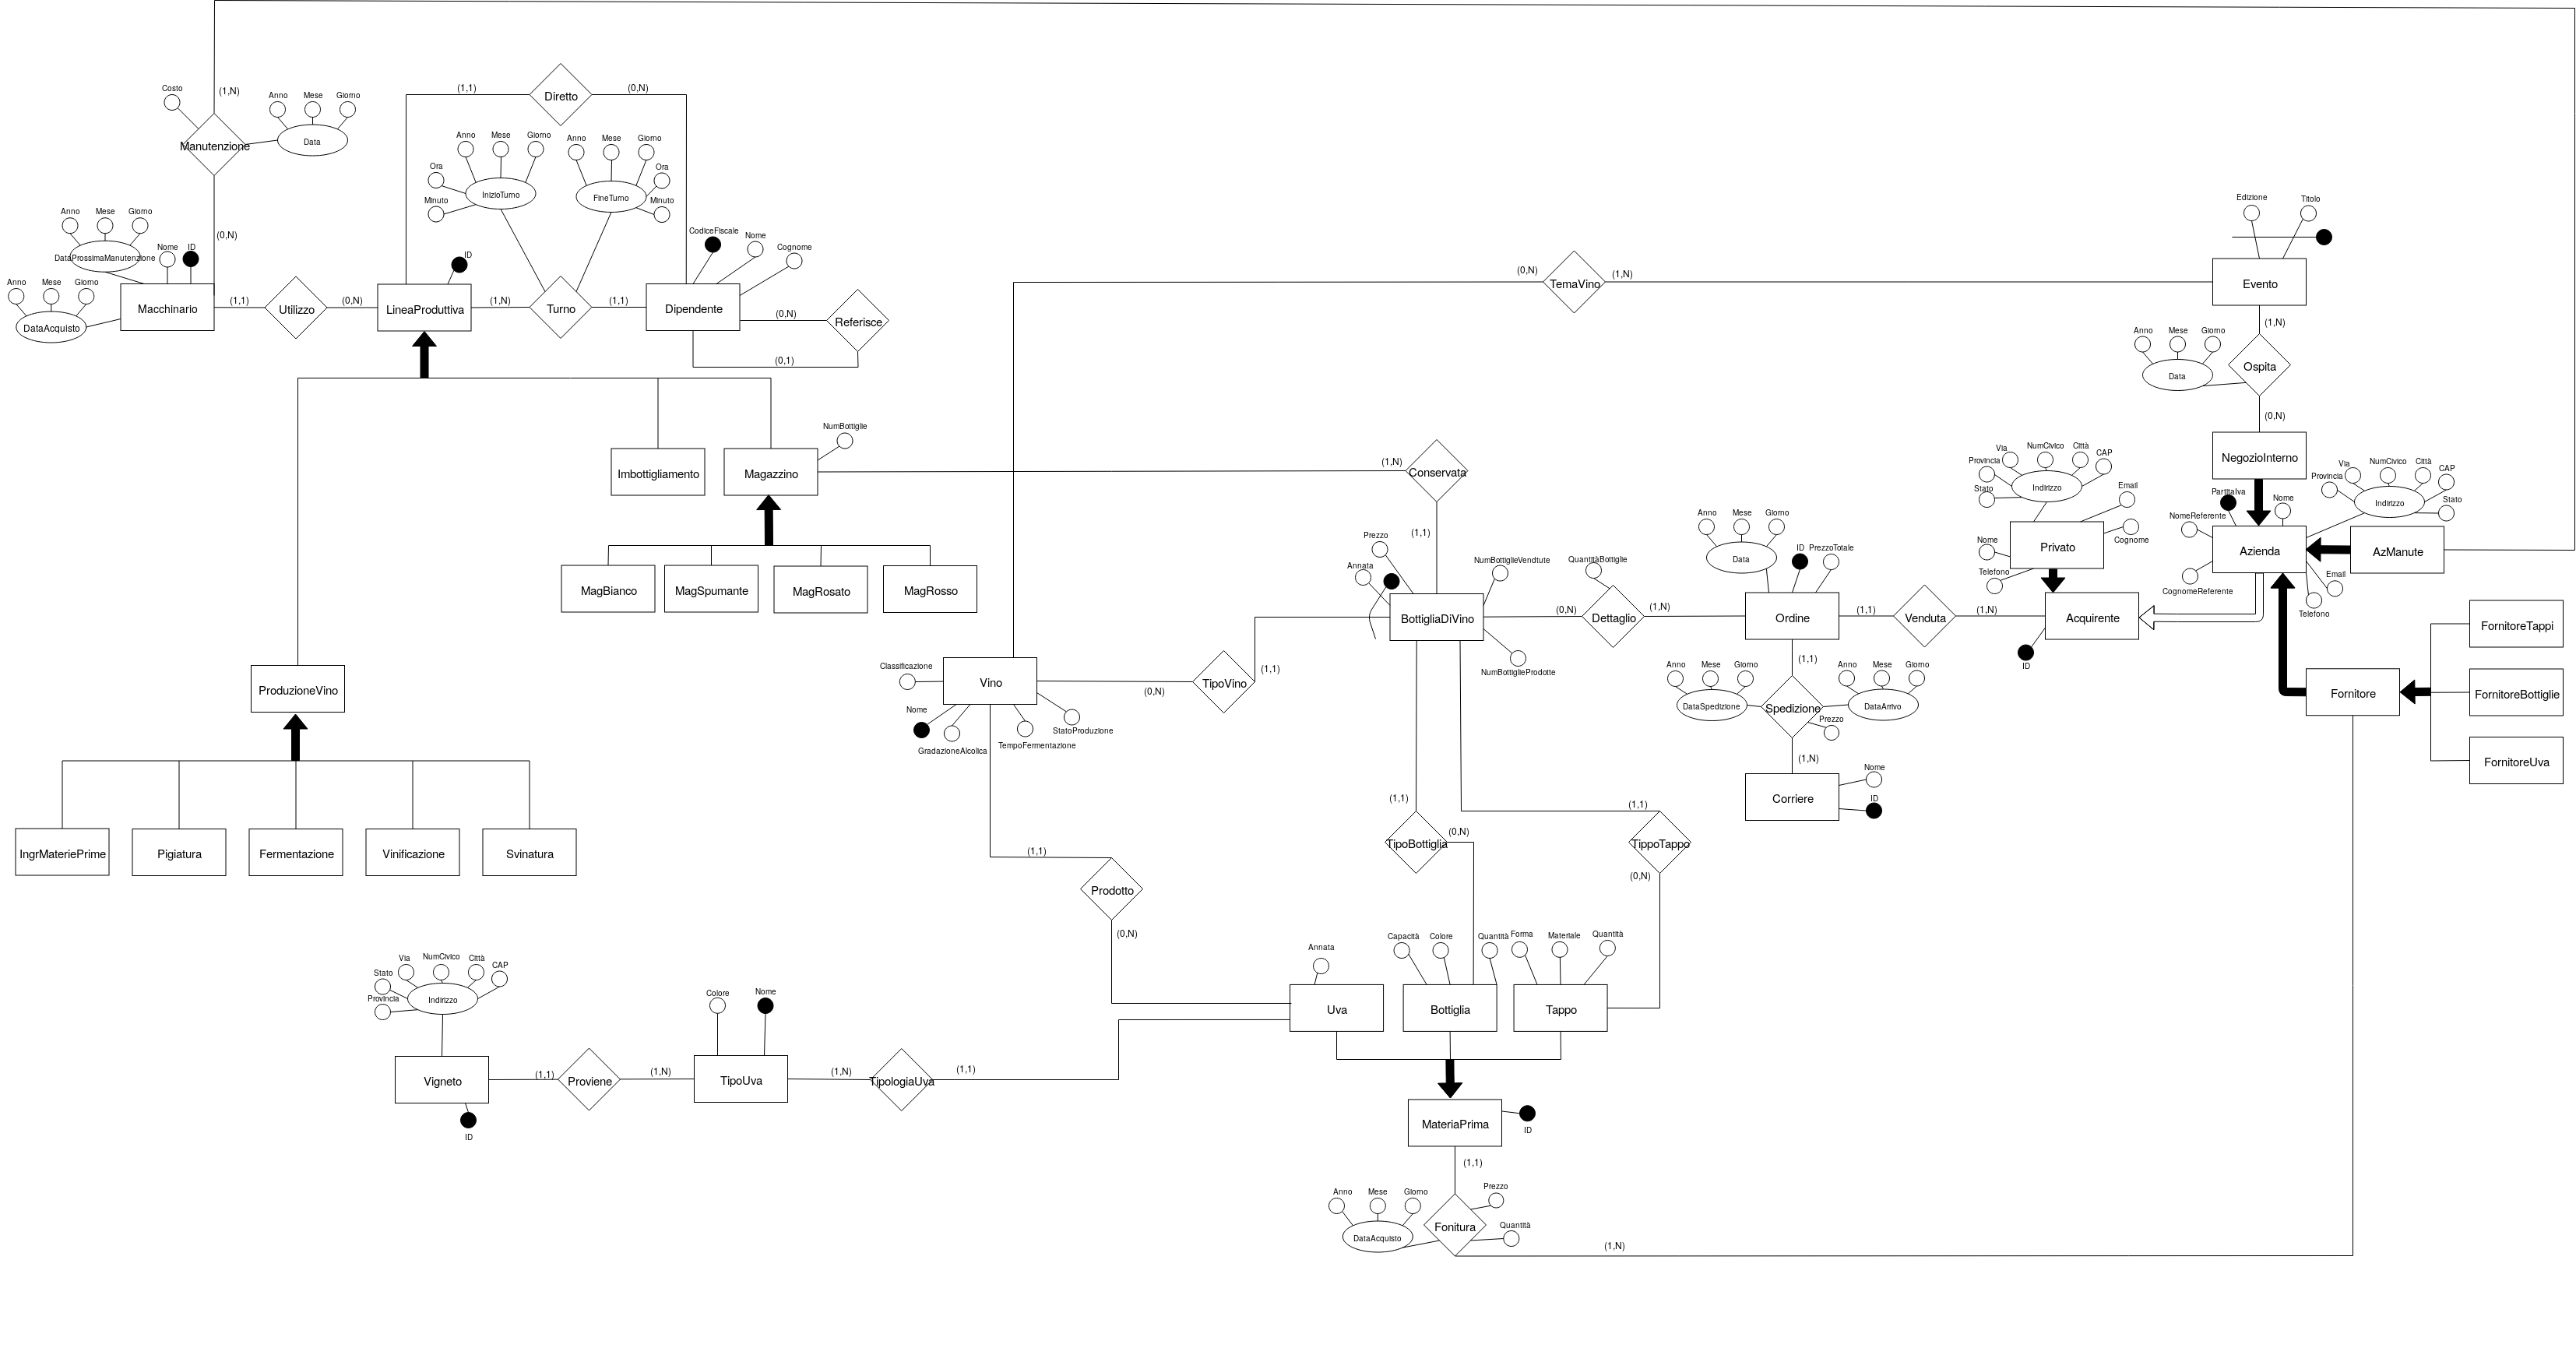
\includegraphics[width=25cm,keepaspectratio,angle=90]{src/progettazioneConcettuale/assests/cantina_ER.png}}
\end{figure}

\section{Progettazione logica}
\subsection{Analisi ridondanze}
	Lo schema concettuale presenta un attributo ridondante, cioè il \textbf{PrezzoTotale} presente nell'entità \emph{Ordine}. Questo attributo è derivabile da $\sum_{n = 1}^{j} (PrezzoBottiglia_n \times Quantita'Bottiglie_n) + PrezzoSpedizione$, 
dove $j$ è il numero di tipologie di bottiglie di vino presenti nell'ordine,
\textbf{PrezzoBottiglia} è l'attributo dell'entità \emph{Bottiglia di vino}, \textbf{PrezzoSpedizione} è l'attributo della relazione \emph{Spedizione} e \textbf{QuantitàBottiglie} è l'attributo della relazione \emph{Dettaglio}. L'operazione coinvolta è la \emph{Stampa resoconto guadagno}, che avviene 1 volta alla settimana. Analizziamo la tavola dei volumi e delle operazioni:

\begin{center}
	\begin{tabular}{P{2cm}P{8cm}P{4cm}}
		\multicolumn{3}{c}{\textbf {\large {Tavola dei volumi}}} \\
		\toprule
		\rowcolor[rgb]{.929, .929, .929} Concetto & Costrutto & Volume \\
		\midrule
		BottigliaDiVino & E & 50\\
		\midrule
		Ordine & E & 350\\
		\midrule
		Corriere & E & 25\\
		\midrule
		Dettaglio & R & 350\\
		\midrule
		Spedizione & R & 350\\
		\bottomrule
	\end{tabular}

	\vspace{0.5cm}

	\textbf{\large{Tavola delle operazioni}}\\
	\vspace{0.2cm}
	\begin{minipage}{6cm}
		\rightline{
			\begin{tabular}{P{2cm}P{2cm}P{1.1cm}P{1cm}}
				\multicolumn{4}{c}{\textbf {Con ridondanza}} \\
				\toprule
				\rowcolor[rgb]{.929, .929, .929} Concetto & Costrutto & Accesso & Tipo \\
				\midrule
				BottigliaDiVino & E & 0 & -\\
				\midrule
				Ordine & E & 1 & L\\
				\midrule
				Dettaglio & R & 0 & -\\
				\midrule
				Spedizione & R & 0 & -\\
				\bottomrule
			\end{tabular}
		}
	\end{minipage}
	\hspace{2mm}
	\begin{minipage}{6cm}
		\leftline{
			\begin{tabular}{P{2cm}P{2cm}P{1.1cm}P{1cm}}
				\multicolumn{4}{c}{\textbf {Senza ridondanza}} \\
				\toprule
				\rowcolor[rgb]{.929, .929, .929} Concetto & Costrutto & Accesso & Tipo \\
				\midrule
				BottigliaDiVino & E & 350 & L\\
				\midrule
				Ordine & E & 1 & L\\
				\midrule
				Dettaglio & R & 350 & L\\
				\midrule
				Spedizione & R & 350 & L\\
				\bottomrule
			\end{tabular}
		}
	\end{minipage}

\end{center}

\begin{flushleft}
In questo esempio vediamo che nello schema \emph{con ridondanza} viene effettuato 1 accesso e 350 letture a settimana alla tabella \emph{Ordini} per ottenere il resoconto settimanale (semplice somma di tutti i prezzi totali degli ordini di una specifica settimana).\\
\vspace{0.5cm}
Nello schema \emph{senza ridondanza}, invece, per ogni ordine occorrera' accedere alle seguenti tabelle:
\begin{itemize}
	\item \emph{BottiglieDiVino} per conoscere il prezzo della singola bottiglia dell'ordine;
	\item \emph{Spedizioni} per conoscere il prezzo della spedizione;
	\item \emph{Dettagli} per conoscere il prezzo totale delle bottiglie acquistate.
\end{itemize}
Si avranno $(350\times3)\times350$, dove $(350\times3)$ sono gli accessi totali alle tre tabelle citate prima e 350 sono le letture della tabella \emph{Ordini}. In totale si avranno $367500$ letture.\\
\begin{verse}
	Alla luce dei risultati emersi della precedente analisi si e' deciso di mantenere l'attributo \textbf{Prezzo totale} in \emph{Ordini}.
\end{verse}
\end{flushleft}

	
\subsection{Eliminazioni generalizzazioni}
Lo schema concenttuale presenta molte generalizzazioni. Si procede all'analisi di quest'ultime per permettere la traduzione verso lo schema logico.\\

\begin{flushleft}
\textbf{\large{Fornitore}}\\
L'entità \emph{Fornitore} presenta solo un attributo comune a tutte le entità figlie, cioè l'identificatore \textbf{ID}. Inoltre l'entità padre \emph{Fornitore} non presenta nessuna relazione con nessun' altra e entità, cose che invece avviene per tutte e tre le entità figlie. Essendo una generalizzazione completa si è deciso di aggiungere l'attributo \textbf{ID} alle entità figlie \emph{FornitoreUva, FornitoreTappi, FornitoreBottiglie} e di eliminare l'entità padre \emph{Fornitore}. 
\end{flushleft}


\begin{flushleft}
	\textbf{\large{Acquirente}}\\
	L'entità \emph{Acquirente} presenta molteplici attributi ed una relazione. A loro volta anche le entità figlie \emph{Azienda e Privato} hanno attributi significativi. Per ristrutturare questa generalizzazione si è deciso di creare due relazioni differenti. La prima si chiama \textbf{IsAzienda} dove la cardinalità in entrambi i versi è di (1,1), cioè un' acquirente può essere solo un' azienda, ed un' azienda è identificata come un solo acquirente.
	La seconda relazione si chiama \textbf{IsPrivato} dove le cardinalità sono rappresentate come fra \emph{Azienda ed Acquirente}. Le entità \emph{Azienda e Privato} avranno sempre gli attributi visti in precedenza ed inoltre l'attributo \textbf{ID} che ha il ruolo di chiave primaria e di chiave referenziale con l'attributo \textbf{ID} di \emph{Acquirente}. 
\end{flushleft}

\begin{flushleft}
	\textbf{\large{Azienda}}\\
	L'entità \emph{Azienda} può essere un negozio interno della cantina. Per ristruttrua questa generalizzazione si è deciso di aggiungere un attributo BOOLEAN all'entità \emph{Azienda} chiamato  \textbf{IsNegozioInterno} (visto che \emph{NegozioInterno} non ha nessun attributo) che va ad identificare se l'azienda è effettivamente un negozio della cantina. Bisogna quindi prestare attenzione all'organizzazione di eventi che possono essere ospitati solo da aziende che sono negozi interni, e che quindi hanno l'attributo  \textbf{IsNegozioInterno} settato a TRUE.
\end{flushleft}

\begin{flushleft}
	\textbf{\large{LineaProduttiva}}\\
	L'entità \emph{LineaProduttiva} è una generalizzazione a più livelli, infatti essa generalizza le entità \emph{ProduzioneVino, Imbottigliamento, Magazzino}. A sua volta l'entità \textbf{ProduzioneVino} generalizza \emph{IngrMateriePrime, Pigiatura, Fermentazione, Vinificazione, Svinatura}. Essendo tutte generalizzazione complete e non avendo attributi (a parte l'entità \emph{Magazzino}*) che vanno a particolarizzare le varie entità figlie, si è deciso di aggiungere un attributo \textbf{Tipologia} nell'entità \emph{LineaProduttiva} che identifica queste specializzazioni.
\end{flushleft}

\begin{verse}
	*L'attributo \textbf{NumBottiglie} dell'entità \emph{Magazzino}, essendo di cardinalità (1,1) per l'entità \emph{BottigliaDiVino}, è stato assegnato a quest'ultima perchè viene identificato univocamento per ogni tipologia di bottiglia di vino.
\end{verse}

\subsection{Partizionamento/accorpamento di entità e relationship}
\textbf{\large{Informazione}}\\
Si è deciso di aggiungere l'entità \emph{Informazione} in modo da raggruppare le (numerose) informazioni comuni delle entità \emph{Privato} ed \emph{Azienda} . L'entità \emph{Informazione} contiene quindi gli attributi \textbf{ID (VARCHAR), Email (VARCHAR), Telefono (VARCHAR), Nome (VARCHAR)}, i quali vengono rimossi dalle sopracitate entita'.

\begin{flushleft}
\textbf{\large{Indirizzo}}\\
Si è deciso di aggiungere l'entità \emph{Indirizzo} in modo da raggruppare le informazioni dell'attributo \textbf{Indirizzo} di \emph{Informazione} e \emph{Vigneto}. L'entità \emph{Indirizzo} contiene quindi gli attributi \textbf{ID (VARCHAR), Stato (VARCHAR), Città (VARCHAR), Provincia (VARCHAR), CAP (INTEGER), Via (VARCHAR), NumCivico (INTEGER)}, i quali vengono rimossi dalle sopracitate entita'.
\end{flushleft}

\begin{flushleft}
\textbf{\large{Date, InizioTurno, FineTurno}}\\
\textbf{InizioTurno, FineTurno} e piu' generalmente qualsiasi entita' \textbf{\emph{Data}} e' stata trasformata in un attributo singolo e rappresentata attraverso il tipo \textbf{DATE} o \textbf{DATETIME}.
\end{flushleft}


\subsection{Scelta degli identificatori principali}
Oltre agli identificatori visti nella sezione~\ref{analisi_entita}, sono stati aggiunti nuovi identificatori primari:

\begin{itemize}
	\item Si è deciso di aggiungere l'attributo \textbf{ID} (che funge da chiave primaria e referenziale con l'attributo \textbf{ID} di \emph{Azienda}) all' entità \emph{Fornitore};
	\item All'entità \emph{Privato} è stato aggiunto l'attributo \textbf{ID} che ha il ruolo di chiave primaria e di chiave referenziale con l'attributo \textbf{ID} di \emph{Acquirente};
	\item L'entità \emph{NegozioInterno} possiede un attributo \textbf{ID} che e' chiave primaria e chiave referenziale con l'attributo \textbf{ID} di \emph{Azienda};
	\item L'entità \emph{Informazione} appena aggiunta ha come chiave primaria l'attributo \textbf{ID}
	\item L'entità \emph{Indirizzo} appena aggiunta ha come chiave primaria l'attributo \textbf{ID} che e' anche chiave referenziale con l'attributo \textbf{ID} di \emph{Informazione o Vigneto};
	\item E' stato aggiunto l'attributo \textbf{ID}, che e' chiave primaria, a \emph{Uva, Tappo, Bottiglia, Evento} per rendere più semplice le relazioni con queste entità.
\end{itemize}

\subsection{Schema logico-relazionale e vincoli d'integrità referenziale}
\textbf{BottiglieDiVino} (\underline{Id}, Vino, Annata, Prezzo, Classificazione, NumBottiglieVendute, NumBottiglieMagazzino, NumBottiglieProdotte, IdTappo, IdBottiglia, IdMagazzino)
\begin{verse}
	(BottiglieDiVino.Vino, BottiglieDiVino.Annata) $\to$ (Vini.Nome, Vini.Uva.Annata)*\\
	BottiglieDiVino.IdTappo $\to$ Tappi.Id\\
	BottiglieDiVino.IdBottiglia $\to$ Bottiglie.Id\\
	BottiglieDiVino.IdMagazzino $\to$ LineeProduttive.Id
\end{verse} 
\textbf{Vini} (\underline{Nome}, GradazioneAlcolica, TempoFermentazione, StatoProduzione, Uva)
\begin{verse}
	Vini.Uva $\to$ Uva.Id
\end{verse} 
\textbf{Uva} (\underline{Id}, TipoUva, Fornitore, Annata)
\begin{verse}
	Uva.Fornitore $\to$ Fornitori.Id\\
	Uva.TipoUva $\to$ TipiUva.Nome
\end{verse}
\textbf{TipiUva} (\underline{Nome}, Colore)\\
\textbf{Vigneti} (\underline{Id}, Indirizzo, TipoUva)
\begin{verse}
	Vigneti.Indirizzo $\to$ Indirizzi.Id\\
	Vigneti.TipoUva $\to$ TipiUva.Nome\\
\end{verse} 
\textbf{Tappi} (\underline{Id}, Forma, Materiale, Quantita, Fornitore)
\begin{verse}
	Tappi.Fornitore $\to$ Fornitori.Id
\end{verse}
\textbf{Bottiglie} (\underline{Id}, Capacita, Colore, Quantita, Fornitore)
\begin{verse}
	Bottiglie.Fornitore $\to$ Fornitori.Id
\end{verse}
\textbf{FornisceUva} (\underline{Uva, DataAcquisto}, Prezzo, Quantita)
\begin{verse}
	FornisceUva.Uva $\to$ Uva.Id
\end{verse}
\textbf{FornisceTappo} (\underline{Tappo, DataAcquisto}, Prezzo, Quantita)
\begin{verse}
	FornisceTappi.Tappo $\to$ Tappi.Id
\end{verse} 
\textbf{FornisceBottiglia} (\underline{Bottiglia, DataAcquisto}, Prezzo, Quantita)
\begin{verse}
	FornisceBottiglia.Bottiglia $\to$ Bottiglie.Id
\end{verse} 
\textbf{LineeProduttive} (\underline{Id}, Nome, Direttore)
\begin{verse}
	LineeProduttive.Direttore $\to$ Dipendenti.CodiceFiscale
\end{verse} 
\textbf{Macchinari} (\underline{Id}, Nome, DataProssimaManutenzione, DataAcquisto, LineaProduttiva)
\begin{verse}
	Macchinari.LineaProduttiva $\to$ LineeProduttive.Id
\end{verse} 
\textbf{Manutenzioni} (\underline{Id}, Macchinario, Azienda, Costo, Data)
\begin{verse}
	Manutenzioni.Macchinario $\to$ Macchinari.Id\\
	Manutenzioni.Azienda $\to$ Aziende.Id
\end{verse}
\textbf{Dipendenti} (\underline{CodiceFiscale}, Nome, Cognome, Referente)
\begin{verse}
	Dipendenti.Referente $\to$ Dipendenti.CodiceFiscale
\end{verse} 
\textbf{Turni} (\underline{Dipendente, InizioTurno}, FineTurno, LineaProduttiva)
\begin{verse}
	Turni.Dipendente $\to$ Dipendenti.CodiceFiscale\\
	Turni.LineaProduttiva $\to$ LineeProduttive.Id
\end{verse} 
\textbf{Ordini} (\underline{Id}, PrezzoTotale *, Data, Acquirente)
\begin{verse}
	Ordini.Acquirente $\to$ Acquirenti.Id
\end{verse} 
\textbf{Dettagli} (\underline{Ordine, Vino}, QuantitaBottiglie)
\begin{verse}
	Dettagli.Ordine $\to$ Ordini.Id\\
	Dettagli.Vino $\to$ BottiglieDiVino.Id
\end{verse} 
\textbf{Spedizioni} (\underline{Ordine, Corriere}, DataSpedizione, DataConsegna, Prezzo)
\begin{verse}
	Spedizioni.Ordine $\to$ Ordini.Id\\
	Spedizioni.Corriere $\to$ Corrieri.Id
\end{verse} 
\textbf{Corrieri} (\underline{Id}, Nome)\\
\textbf{Acquirenti} (\underline{Id})\\
\textbf{Privati} (\underline{Id}, Cognome, InformazioniAggiuntive)
\begin{verse}
	Privati.Id $\to$ Acquirenti.Id\\
	Privati.InformazioniAggiuntive $\to$ Informazioni.Id
\end{verse} 
\textbf{Aziende} (\underline{Id}, NumAcquirente, PartitaIva, NomeReferente, CognomeReferente, InformazioniAggiuntive)
\begin{verse}
	Aziende.NumAcquirente $\to$ Acquirenti.Id\\
	Aziende.InformazioniAggiuntive $\to$ Informazioni.Id
\end{verse}
\textbf{Fornitori} (\underline{Id}, Tipologia)
\begin{verse}
	Fornitori.Id $\to$ Aziende.Id
\end{verse} 
\textbf{NegoziInterni} (\underline{Id})
\begin{verse}
	NegoziInterni.Id $\to$ Aziende.Id
\end{verse} 
\textbf{Indirizzi} (\underline{Id}, Via, NumeroCivico, Stato, Provincia, Citta, CAP)\\
\textbf{Eventi} (\underline{Id}, Titolo, Edizione)\\
\textbf{Ospita} (\underline{Evento, Negozio}, Data)
\begin{verse}
	Ospita.Evento $\to$ Eventi.Id\\
	Ospita.Negozio $\to$ NegoziInterni.Id
\end{verse}  
\textbf{TemiVino} (\underline{Vino, Evento})
\begin{verse}
	TemiVino.Vino $\to$ Vini.Nome\\
	TemiVino.Evento $\to$ Eventi.Id
\end{verse}
\textbf{Informazioni} (\underline{Id}, Nome, Telefono, Email, Indirizzo)
\begin{verse}
	Informazioni.Indirizzo $\to$ Indirizzi.Id
\end{verse}


\begin{verse}
	*\emph{Per ovviare al problema del vincolo referenziale fra \textbf{BottiglieDiVino.Annata e Vini.Uva.Annata} e \textbf{Ordini.PrezzoTotale} come somma di \begin{math}(BottiglieDiVino.Prezzo \times Dettagli.QuantitaBottiglie)+ Spedizioni.Prezzo\end{math}} si potrebbe aggiungere un \textbf{TRIGGER}, cosa comunque non richiesta ai fini del progetto.
\end{verse}

\section{Query ed indici}
\subsection{Query}
\begin{enumerate}
	\item \textbf{Bottiglia/e di vino più venduta/e dell'anno 2019 con la relativa quantità}
	\item \textbf{Numero di tipi di vino prodotti divisi per colore}
	\item \textbf{Coppie di aziende che hanno acquistato lo stesso giorno, con il relativo giorno, in ordine alfabetico}
	\item \textbf{Lista dei dipendenti (nome, cognome), con inizio e fine turno, ordinati in modo decrescente sull'inizio del turno, che sono a lavorare il giorno 12 giugno 2019}
	
\end{enumerate}\label{stampa_resoconto_guadagno}

\subsection{Indici}
E' opportuno creare un indice sulla tabella \emph{Dipendenti} perchè analizzando il carico della base di dati, tale tabella contiene dati che vengono acceduti spesso in lettura ma non in scrittura. L'unico momento in cui la tabella viene acceduta in scrittura è in concomitanza all'assunzione di nuovi dipendenti, azione svolta solamente 10 volte l'anno.
\begin{flushleft}
	\textbf{{Creazione indice:}} \emph{CREATE INDEX idx\_dipendenti ON Dipendenti (CodiceFiscale)}
\end{flushleft}

\begin{minipage}{6cm}
	\rightline{
		\centering
		\textbf{Esecuzione senza indice}
		%inserimento immagine
	}
\end{minipage}
\hspace{2mm}
\begin{minipage}{6cm}
	\leftline{
		\centering
		\textbf{Esecuzione con indice}
		%inserimento immagine
}
\end{minipage}
\end{document}